\documentclass{article}
\usepackage{amsmath}
\usepackage{amssymb}
\usepackage{bbm}
\usepackage{graphicx}
\usepackage[margin=1in]{geometry}
\renewcommand{\P}P
\newcommand{\T}T
\renewcommand{\t}t
\newcommand{\x}X
\newcommand{\p}p
\newcommand{\n}n
\newcommand{\m}m
\renewcommand{\c}c
\newcommand{\posorthant}{R^n_+}
\newcommand{\simp}[1][]{\Delta^{#1}}
\DeclareMathOperator{\diag}{diag}
\begin{document}


Exact, nonparametric confidence interval for incidence given repeated measurements


literature:
overviews of exact, small sample methods for contingency table data:
1. Mehta CR. The exact analysis of contingency
tables in medical research. Statistical Methods
in Medical Research 1994; 3: 135–56.
2. Agresti A. Exact inference for categorical data: Recent advances and continuing controversies.
Statistics in Medicine 2001; 20: 2709–22

\section{Method}

\subsection{Data}
The data are $n$ IID vectors of length
$m$ consisting of binary values, 
$$
(\x_{11},\x_{12},\ldots,\x_{1m}), (\x_{21},\x_{22},\ldots,\x_{2m}), \ldots,
(\x_{n1},\x_{n2},\ldots,\x_{nm}), \x_{ij}\in\{0,1\}.
$$ We don't make any assumptions about
the dependence structure within each vector
$(\x_{i1},\x_{i2},\ldots,\x_{im})$. The sums
$\sum_{j=1}^m\x_{ij}, i=1,\ldots,n$ are IID. Since each $\x_{ij}$ is
$0$ or $1$, the sums are IID random variables each taking a value in
$0,1,\ldots,m$. Viewing $0,1,\ldots,m$ as $m+1$ categories, we can
identify each vector sum $\sum_{j=1}^m\x_{ij}$ as a choice of
one of thse $m+1$ categories% , with the weights determined by the
% unknown marginal probabilities of the vector components
. These choices
are IID, so their sum is multinomial. ((rewrite $m$ to $m-1$ to be
consistent with the remainder?))

\subsection{Multinomial estimation}

Let $\x_0$ be an observaiton from the multinomial distribution with
sample size $\n$ and parameter $\p_0% =(\p_,\ldots,\p_m)
$. Let
$\c=(0,\ldots,\m-1)/(\m-1)$. The goal is a confidence interval for
$\theta_0=\c^t\p_0$ based on $\x_0$.

One CI is given by maximum likelihood. The MLE $\c^t\hat\p$ is asymptotically
normal with variance $\c^t(\diag(\p)-\p\p^t)\c$, which may be approximated by $\c^t(\diag(\hat\p)-\hat\p\hat\p^t)\c$. For a
given finite sample size, the coverage of this CI deteriorates as the
multinomial parameter $\p$ approaches the boundary of the parameter
space, the simplex in $R^m$. We therefore look for a more efficient
CI.

We may obtain an exact CI by inverting a hypothesis test. % Let a
% hypothesis test based on the sample $\x_0$ that the null parameter is
% $\theta$ be given by a test statistic $\T(\x_0,\theta)$ that rejects for
% large values. As the null $\theta=\{\p\in \Delta^{m-1}:\c^t\p=\theta\}$ is composite, the test rejects at level $\alpha$ when
% \begin{align}
%  \sup_{p:\c^tp=\theta}\P_\p(\T(\x,\p)\ge\T(\x_0,p))<\alpha
% \end{align}((inconsistent--T based on p or theta?))
% $\T=\T(\x,\p)$ is a function of the data $\x$ and a
% parameter value $\p$. A test of the null that $\x$ is distributed as
% $\p$ rejects for large values of $\T$. Choices
% of $\T$ discussed below. The set of parameters $\p$ at which the test fails to reject,
% \begin{align}
%   A(\x_0)=\{\p : \P(\T(\x,\p)\ge\T(\x_0,p)\mid \x_0)\ge\alpha
%   \text{ where }\x\sim\p\}
% \end{align}
% contains $\p_0$ with probability $\ge 1-\alpha$,
% \begin{align}
%   % &\P(\p_0 \in \{\p' : \P(\T(\x,\p')\ge\T(\x_0,p'))\ge\alpha
%   % \text{ where }\x\sim\p'\})\\
%   &\P(\p_0\in A(\x_0))\\
%   &=\P(\P(\T(\x,\p_0)\ge\T(\x_0,\p_0)\mid\x_0)\ge\alpha
%     \text{ where }\x\sim\p_0)\\
%     &=\P(\T(\x_0,\p_0)\text{ is $\le$ the $1-\alpha$ quantile of $\T(\x,\p_0)$, where} \x,\x_0\sim\p_0)
%       &\ge 1-\alpha
% \end{align}
% ((equality when the $1-\alpha$ quantile is unique eg CDF is continuous))
% The set ((ref)) may therefore serve as a CI for $\p_0$. A CI for the composite null  $\theta_0=\{\p\in \Delta^{m-1}:\c^t\p=\theta_0\}$ is given by
% \begin{align}
%   \{\theta : \sup_{p:\c^tp=\theta}\P_{\x\sim\p}(\T(\x,\p)\ge\T(\x_0,p)\mid\x_0)> \alpha\}.
% \end{align}

$\T=\T(\x,\p)$ is a function of the data $\x$ and a parameter value
$\p$. Choices of $\T$ discussed below. A level $\alpha$ test of the
null that $\x_0$ follows $\p$ rejects for large values of $\T$, i.e.,
$\T(\x_0,\p)\ge t_{\p,\alpha}$, where
$t_{\p,\alpha}=\inf\{t:\P(\T(\x,\p)\ge t)\ge\alpha\}, \x\sim\p,$ is
the $1-\alpha$ quantile of $\T(\x,\p)$ under $\p$. A level $\alpha$
test that $\x_0$ follows a distribution in the composite null
$\theta=\{\p\in \Delta^{m-1}:\c^t\p=\theta\}$ rejects when
$\sup_{\p:\c^t\p=\theta}\T(\x_0,\p)-t_{\p,\alpha}>0$. The set of
parameters $\theta$ at which the test fails to reject,
\begin{align}
  A(\x_0)=\{\theta : \sup_{\p:\c^t\p=\theta}\T(\x_0,\p)-t_{\p,\alpha} \ge 0\}
\end{align}
contains $\theta_0$ with probability $\ge 1-\alpha$,
\begin{align}
  % &\P(\p_0 \in \{\p' : \P(\T(\x,\p')\ge\T(\x_0,p'))\ge\alpha
  % \text{ where }\x\sim\p'\})\\
    &\P(\theta_0\in A(\x_0))\\
    &=\P(\sup_{\p:\c^t\p=\theta_0}\T(\x_0,\p)-t_{\p,\alpha} \ge 0\}\\
  &\ge \P(\T(\x_0,\p_0)\ge t_{\p_0,\alpha} \}\\
  % &=\P(\P(\T(\x,\p_0)\ge\T(\x_0,\p_0)\mid\x_0)\ge\alpha
  %   \text{ where }\x\sim\p_0)\\
  %   &=\P(\T(\x_0,\p_0)\text{ is $\le$ the $1-\alpha$ quantile of $\T(\x,\p_0)$, where} \x,\x_0\sim\p_0)
      &\ge 1-\alpha
\end{align}
((equality when the $1-\alpha$ quantile is unique eg CDF is continuous, when p0 is worse case))
The set ((ref)) may therefore serve as a level $1-\alpha$ CI for $\theta_0$.%  A CI for the composite null  $\theta_0=\{\p\in \Delta^{m-1}:\c^t\p=\theta_0\}$ is given by
% \begin{align}
%   \{\theta : \sup_{p:\c^tp=\theta}\P_{\x\sim\p}(\T(\x,\p)\ge\T(\x_0,p)\mid\x_0)> \alpha\}.
% \end{align}


%
$\T=\T(\x,\p)$ is a function of the data $\x$ and a
% parameter value $\p$. A test of the null that $\x$ is distributed as
% $\p$ (but htis is composite) rejects for large values of $\T$. Choices
% of $\T$ discussed below. A level $\alpha$ confidence interval for
% $\p_0$ is given as $\{\p : \P_\p(\T(\x,\p)\ge\T(\x_0,p))\ge\alpha\}$, where $\x\sim\p$ .((details))
% A level $\alpha$ CI for $\theta_0=\c^t\p_0$ is given by
% \begin{align}
%   \{\theta : \sup_{p:\c^tp=\theta}\P_\p(\T(\x,\p)\ge\T(\x_0,p))\ge\alpha\}
% \end{align}

chioce of T...

Applying this procedure requires the distribution of the test statistic
$(\T(\x,\p)$ at $\p$, which is often unavailable. We approximate, to arbitrary accuracy, by
using a sample observed distribution, i.e., sampling $\T(\x,\theta)$
under $\p$.

This sampling at each $\p$ in turn requires a choice of $\p$, and
therefore $\theta$ values to be selected as candidates. We approximate
the supremum in ... by choosing a subset of $\{\p:\c^t\p=\theta\}$,
for a subset of the possible values of
$\theta\in[\min_i\c_i,\max_i\c_i]$. Two further tuning parameters are
introduced, controlling the number of $\theta$ and the number of $\p$
at each $\theta$. ((may vary by $\theta$ to reflect prior knowledge)) Obtaining a subset of $\{\p:\c^t\p=\theta\}$ is described below.

This CI is exact, i.e., its mean coverage equals the nominal coverage, subject to provisos:
\begin{enumerate}
\item monte carlo error, which may be reduced arbitrarily by increasing the tuning parameters ...
\item the null hypothesis $\theta=\theta_0=\{\p : \c^t\p=\theta_0\}$
  is a composite null hypothesis, so that the test statistic on which
  the CI is based is conservative. That is, the null consists of
  multiple distributions and the p-value is the least favorable ((ref
  supremum above)). This is part of the definition of a p-value and
  unavoidable due to the equivalence of CIs and hypothesis
  testing. Difference is the gap between largest and smallest p-values
  within a $\theta$ section, which in turn depends on the choice of test statistic, sample size, number of categories. In simulations below, the effect is to
  inflate the coverage by $<1\%$.
\item discreteness. There are $m^n$ possible values for $X$ sampled as
  multinomial of size $n$ with $m$ categories, so at most $m^n$
  possible values for a test statistic $T$. Often fewer observed
  values when $p$ is close to the boundary of the simplex and some
  categories are rarely observed. Therefore at most $m^n+1$ possible
  values for a p-value.  The nominal level of the test may not be
  among these p-values, in which case the p-value that is used will be
  larger than the nominal level. This issue may be addressed by
  introducing randomness to the test statistic ((Stevens WL. Fiducial
  limits of the parameter of a discontinuous distribution. Biometrika
  1950; 37: 117–29)), though in practice doing so is ``considered
  unacceptable'' ((lehmann romano)), instead using p-values which are
  among those made available by the data. ((agresti 2003 stat meth for
  for overview of discreteness leading to conservative CIs for count data.))
\end{enumerate}
((agresti 2003 definition of ``exact'' is that the CI is based on a
test stat the distirbution of which is known exactly and not
asymptotically or otherwise approximate. This definition applies here
other up to the monte carlo error, which is under the control of the
analyst. Under the Agresti definition, an exact CI for count data is typically
conservative, as in our case, due to discreteness. A further issue in our case is that the null hypotheses, on which the CI is constructed, is compound.))


\subsection{Algorithm}

algorithm:

1. select theta values. remark: can take a grid, or sample. can choose to reflect prior knowledge. if only interested in testing the null of a specific theta value, can just take one value.

2. at each theta value:

2a. sample p values in preimage of theta. remark
similar to above. dirichlet sparsity/concentration.

2a. at each p value: for empirical cdf of test stat. use to get a
p-value at this p.

2b. take max to get a pval associated with this theta. remark:
conservative. max of the observations (over time: expectation of the
max) being used as an estimate of the max of the expectations. requires coordination between number of smaples in 2b, controlling how close the p-value estimates are to the true pvalue, and the number of p values selected in 2a.

3. $1-\alpha$ CI for theta can be constructed as those theta for which the associated p-value exceed $\alpha$.


((maybe mention original algorithm, sampling p first, add sims in appendix))


details for 2a:

describe sampling procedure. The hyperplane $c^tx=1$ in $\{x\ge 0\}\subset\mathbb{R}^m$, for constant $c\ge 0$, is contained in $[0,c_1^{-1}]\times\ldots\times[0,c_m^{-1}]$. So can use rejection sampling to sample points uniformly on its intersection with the solid simplex. Then transform ... to probability simplex. Acceptance probability $O(1/m!)$ (volume of solid simplex in $\mathbb{R}^m$).

More efficient sampling procedures.

approach 1. fast but not uniform sampling. we want to sample from the
intersection of the probability simplex
$\mathbbm{1}^tx=1, 0\le x\le 1,$ and the hyperplane $\c^t x=1$ for a
coefficient vector $\c$. In our application $\c= ...$. These points
satisfy $c^t x=1=\mathbbm{1}^t x$ or $(c - \mathbbm{1})^t x = 0$ and
lie in the unit cube. Therefore we sample $u$ on the orthogonal
complement of $c - \mathbbm{1}$ and divide $u$ by
$\sum_i u_i = \sum_i c_iu_i$. give details. The difficulty is that the
central projection, $u\mapsto u/(\sum_i u_i)$ does not preserve
uniformity, so sampling $u$ as uniform on delta cross delta will not
induce a uniform distribution. seems difficult to even identify the
uniform distribution we are want without enumerating the vertices in
the intersection of the simplex and linear subspace.

could try to account for the distortion of the central projection. If
$J$ is its jacobian, then the distribution $\propto ...$ on the
intersection of $\mathbb{R}^m_+$ with the linear subspace $...$ will
lead to a uniform distribution on the intersection of this subspace
with $\Delta^{m=1}$. To normalize the distribution would need to
integrate this form over ((interscton of orthant with lnear
subspace)), itself a vertex enumeration problem. Another possibility
would be to use markov chain monte carlo sampling techniques that only
require the unnormalized density. would require waiting for convergence at each $\theta$.


approach 2. slow but uniformly distributed (can get other distributions too). For $c\ge 0, \theta>0$, the intersection of $\simp[m-1]$
with $\c^tx=\theta$ is a convex polyhedron in $\posorthant$, i.e., the
convex hull of a finite set of vectors
$\{v_1,\ldots,v_k\}\subset\posorthant$. These vectors may be
enumerated in time $...$. Therefore sample uniformly on the
probability simplex $\simp[k-1]$ (e.g., normalized exponentials) and
apply to the sample the linear transformation mapping the standard
basis vector $e_i$ to $v_i$, $i=1,\ldots,k$. Since linear
transformations preserve uniformity ((e.g., devroye)), the image is
uniformly distributed on $\simp[m-1]\cap \{\c^tx=\theta\}$. Can also use other sampling schemes on the probability simplex to reflect prior knowledge about the location of the true parameter. E.g., Dirichlet.




\section{Simulation}

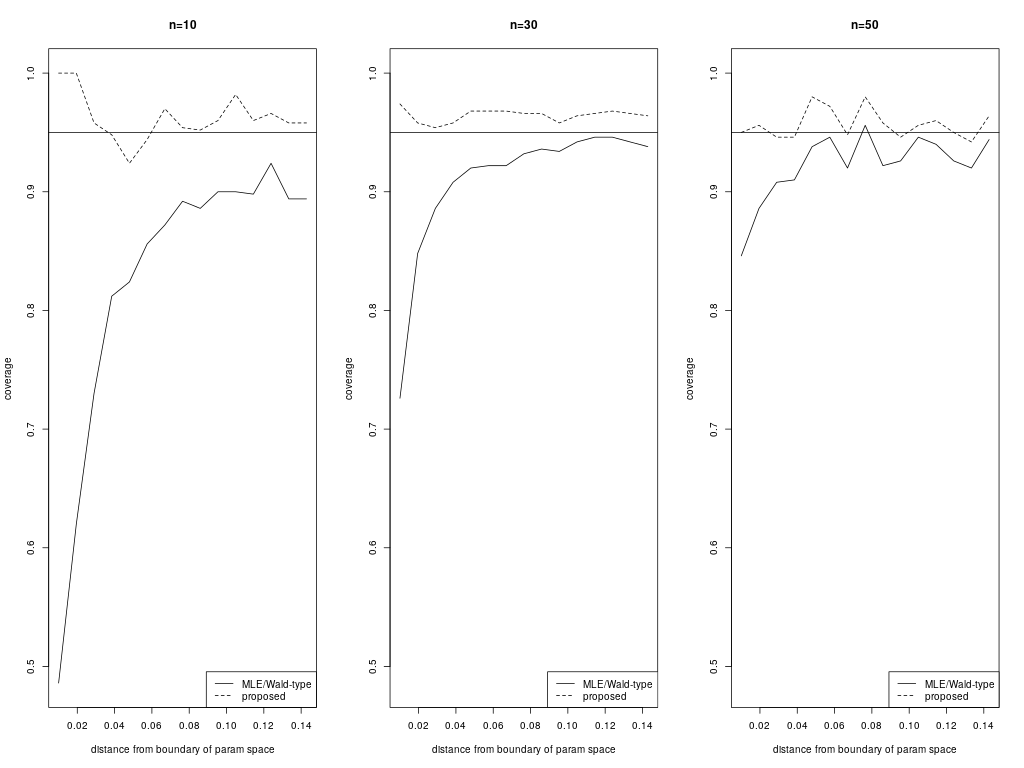
\includegraphics[width=\textwidth]{coverage.png}

give power curves, maybe with different dirichlets

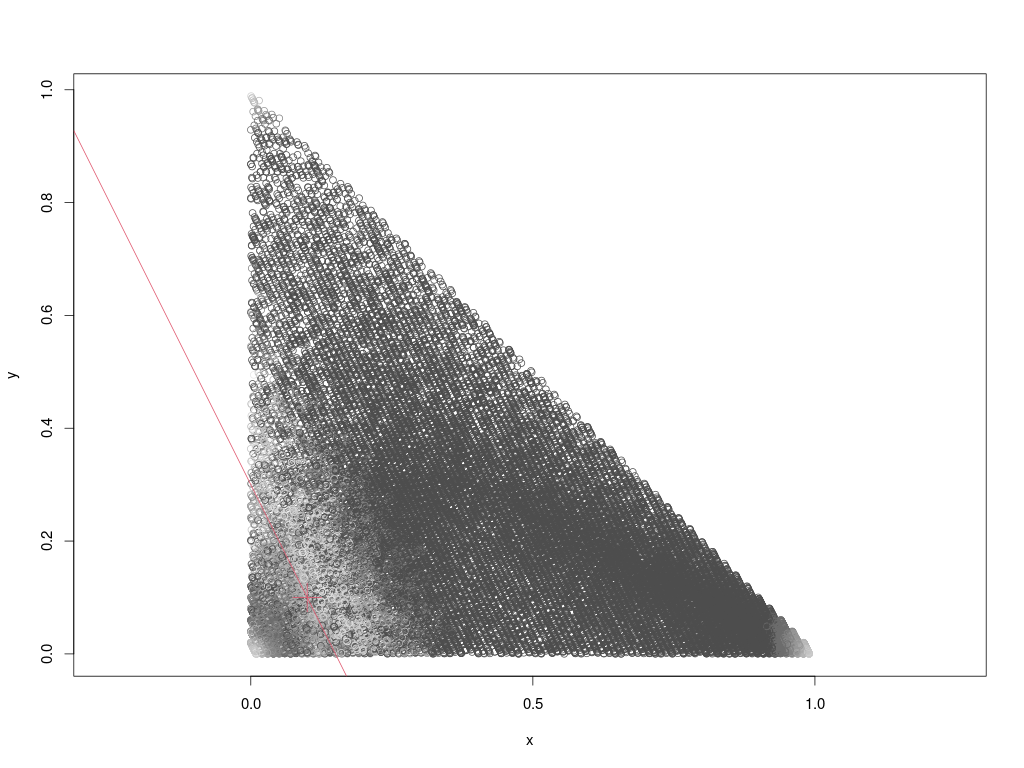
\includegraphics[width=\textwidth]{power.png}
((convert color to bw, set asp ratio to 1, smooth out, legend))
\end{document}


could cache the samples from the reference distributions at each
vector p. assumes that the same data set dimensions are being
used. test statistic is being used.

tried sampling from the preimage of theta. intersection of simplex
with a hyperplane.



Do we need exchangeability? 




